\chapter{SaaS, le teclologie che ne consentono la realizzazione}
Nel corso degli ultimi anni, con il proliferarsi delle piattaforme e dei servizi di Cloud Computing, sono nate e si sono sviluppate molte tecnologie per soddisfare le nuove esigenze e i nuovi requisiti appena visti che questa rivoluzione della fruizione del software ha comportato.

\section{Microservizi}
Un concetto fondamentale, di cui il Cloud Computing fa largamente uso, sono i mircoservizi. Cominciamo col darne una definizione abbastanza formale: "Lo stile architetturale a microservizi è un approccio allo sviluppo di una singola applicazione come insieme di piccoli servizi, ciascuno dei quali viene eseguito da un proprio processo e comunica con un meccanismo snello, spesso una HTTP API.(Martin Fowler)".

\paragraph{}
L'approccio è quello di dividere le funzionalità del sistema in più microservizi. Ad ogni microservizio corrisponde una necessità dell'utente. La filosofia di dividere il software in base alle resposabilità è già presente da tempo nell'ingegneria del software. Una suddivisione modulare del sistema in base ai casi d'uso dell'utente è già presente da tempo nell'Object Oriented Design, ma la novità apportata dai microservizi è che il sistema con essi risulta scomposto in realtà in piccoli servizi completamente indipendenti tra loro. Ogni microservizio si preoccupa infatti di risolvere un particolare problema del cliente, un unico scenario. La comunicazione tra i servizi avviene attraverso la rete al fine di garantire l’indipendenza tra i servizi ed evitare ogni forma di accoppiamento. Ogni microservizio, infatti, rappresenta un'entità separata che generalmente viene pubblicata come un modulo di una Platform as a Service.

\subsection{Il modello monolitico a layer }
Secondo il classico modello a layer le funzionalità vengono suddivise in base al grado di astrazione tra i vari livelli, usando delle tecnologie proprie di ogni livello. Questi sono separati a livello logico e comunicano tra di loro. Con questa architettura però, nonostante ci sia questa suddivisione a strati, il software risulta essere un unico sistema monolitico, sebbene molti componenti possano essere comunque riusabili.

\begin{figure}[h!]
	\centering
	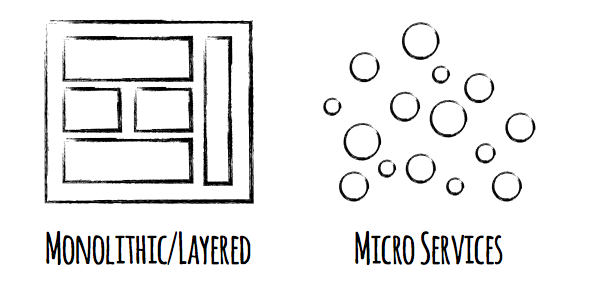
\includegraphics[width=\textwidth,keepaspectratio=true]{capitoli/imgs/disegnoMicrosMonol.png}
	\caption{Il modello monolitico e i microservizi}
\end{figure}

\subsection{Confronto tra l'architettura a microservizi e il modello monolitico}
La scelta di adottare uno o l'altro approccio viene dopo un'attenta analisi dei requisiti che il sistema deve soddisfare. In questo studio però va anche tenuto conto quanto le esigenze possano cambiare nei futuri utilizzi del software.
\begin{itemize}
	\item La struttura interna di tutto un sistema monolitico è composta principalmente dai layer di interfacciamento con l'utente, logica di business e persistenza dei dati. In un'architettura a microservizi non troviamo questa divisione a livello di sistema, ma la ritroviamo semmai all'interno di un singolo microservizio atomico. Ogni microservizio, ad esempio, si occuperà di preservare il suo stato tramite l'utilizzo di un proprio database non condiviso con gli altri microservizi. 
	
	\item Uno dei fattori chiave da considerare è la scalabilità. Per scalare un'applicazione monolitica occorre necessariamente clonarla in più server, macchine virtuali o contenitori.
	
	\item Quando occorre scalare orizzontalmente un'architettura a microservizi, si creano e si distribuiscono indipendentemente tra loro repliche dei microservizi in più server o container. 
\end{itemize}


\begin{figure}[h!]
	\centering
	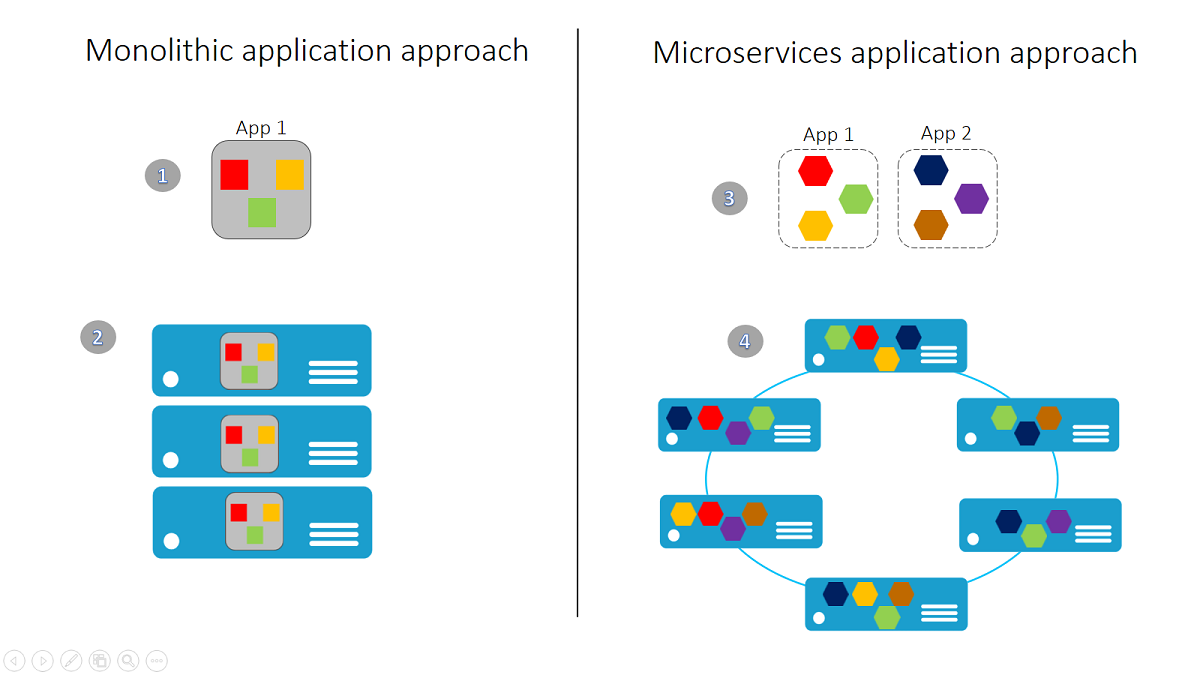
\includegraphics[width=\textwidth,keepaspectratio=true]{capitoli/imgs/monosvmicro.png}
	\caption{Il modello monolitico e i microservizi}
\end{figure}

\subsection{Vantaggi e svantaggi di un'architettura a microservizi}
Un'architettura di questo tipo porta con se ovviamente anche i suoi svantaggi e i suoi vantaggi. Sono proprio questi ultimi che la rendono molto adatta al Cloud Computing.

\subsubsection{Vantaggi}
\begin{itemize}
	\item  Velocità \\
	L'architettura a microservizi è quella che si sposa meglio con la metodologia agile. un microservizio deve avere sempre delle dimensioni ridotte e il suo sviluppo  dovrebbe avere una durata di circa due settimane. Ciò porta ad avere fin da subito piccole porzioni del sistema (i servizi appunto), pronte, testabili ed utilizzabili. Ogni microservizio inoltre è autonomo e può quindi giungere in ambiente di produzione indipendentemente dagli altri. In questo modo si riesce a reagire molto velocemente alle esigenze di mercato.
	
	\item Sperimentazione \\
	Con i microservizi la modularità del sistema è un notevole punto di forza. Sperimentare nuove tecnologie all'interno di un singolo microservizio ha un impatto nullo su tutti gli altri. Si è in questo modo molto più invogliati a ricercare sempre più nuove tecnologie da inserire nel proprio prodotto. Il rischio è minimo in quanto, anche nel caso l'esperienza risulti fallimentare, la mole di lavoro che comporta la modifica di un microservizio e veramente molto ridotta.
	
	\item Tecnologie ad hoc \\
	Altro fattore da considerare è la possibilità di differenziare le tecnologie a seconda del microservizio. Si prenda come esempio la vastità di database che sono disponibili all'uso. Un database che è appropriato per un miocroservizio potrebbe non essere la scelta migliore per un altro. 
	
	\item Scalabilità \\
	I software con un'architettura a microservizi sono pensati per scalare orizzontalmente in maniera estremamente agevole. Si possono replicare a piacimento tramite l'utilizzo di containers e hanno un comportamento distribuito anche nel caso si trovino sulla stessa macchina, in quanto i container li isolano da tutti gli altri.
	
	\item Facilità di Deployment \\
	Le modifiche hanno un impatto molto ridotto nell'interno sistema. Grazie a ciò è possibile rilasciare sul mercato il software aggiornato con frequenze molto maggiori. Potenzialmente ogni modifica può subito essere pubblicata e non occorre attenersi a lunghi processi di release in cui si cerca il più possibile di accumulare modifiche da effettuare per poi applicarle tutte insieme.
	
	\item Portabilità \\
	Il software a microservizi è facilmente componibile e portabile su più contesti e dispositivi, come web,mobile ma anche sistemi embedded o dispositivi indossabili ad esempio.	
\end{itemize}

\subsubsection{Svantaggi}
\begin{itemize}
	\item Dipendenza dalla rete \\
	E' questo il principale punto di critico di un'architettura a microservices. Abbiamo quanto l'interazione tra i singoli microservizi faccia affidamento su una comunicazione attraverso internet. Ovviamente questo deve essere un requisito fondamentale. In mancanza di una connessione adeguata tutto il sistema smette di funzionare.
	
	\item Identità e autenticazione \\
	Una volta che un utente del software effettua il login occorre garantire che la sua autenticazione, e soprattutto la sua identità, venga mantenuta in tutti i microservizi che andranno a comporre la sua esperienza utente.
\end{itemize}

\section{Containers}
I container sono l'habitat naturale dei microservizi. Essi forniscono al software tutto ciò che gli è necessario, garantendogli un ambiente estremamente leggero e flessibile.

\paragraph{}
I containers sono infatti un metodo di virtualizzazione del sistema operativo che ha come obiettivo quello di isolare il software che ospita, permettendo di eseguire le applicazioni e le loro dipendenze in processi completamente isolati. L'infrastruttura del container interagisce direttamente con il kernel della macchina che lo ospita, scavalcando gli altri layer. In qualsiasi sistema operativo collochiamo il container, le sue configurazioni interne rimarranno sempre separate, e l'applicazione contenuta avrà garantito il suo ecosistema necessario all'esecuzione. Non ci si deve preoccupare, ad esempio, di produrre una versione software per Windows e una per sistemi UNIX, ma la soluzione a container e unica e portabile. 

\begin{figure}[h!]
	\centering
	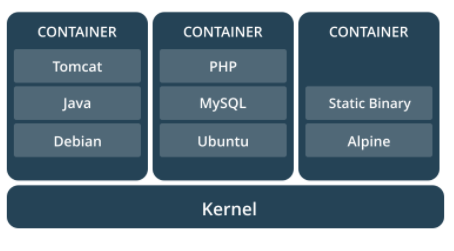
\includegraphics[width=\textwidth,keepaspectratio=true]{capitoli/imgs/container.PNG}
	\caption{Schematizzazione di tre container sulla stessa macchina ospitante}
\end{figure}

\subsection{I containers e le Macchine Virtuali}
Stando alla descrizione dei container che abbiamo dato fino a questo punto potrebbe sorgere una domanda: perchè utilizzare i container se potrebbero essere usate delle macchine virtuali? Una Virtual Machine è per sua natura già isolata dalla macchina che la ospita. La risposta sta nella leggerezza d'uso dei container. I container infatti non virtualizzano l'hardware della macchina, ma solamente il layer applicativo, rendendoli più portabili ed efficienti.

\paragraph{}
Non avendo un proprio sistema operativo, il peso di un container e dell'ordine di qualche Megabyte, contro i Gigabyte di una macchina virtuale che sovrappone il proprio sistema operativo a quello della macchina ospitante. A differenza delle macchine virtuali inoltre, i container non necessitano dell'Hypervisor, un componente che svolge delle attività di controllo e coordinamento sulle macchine virtuali. 

\begin{figure}[h!]
	\centering
	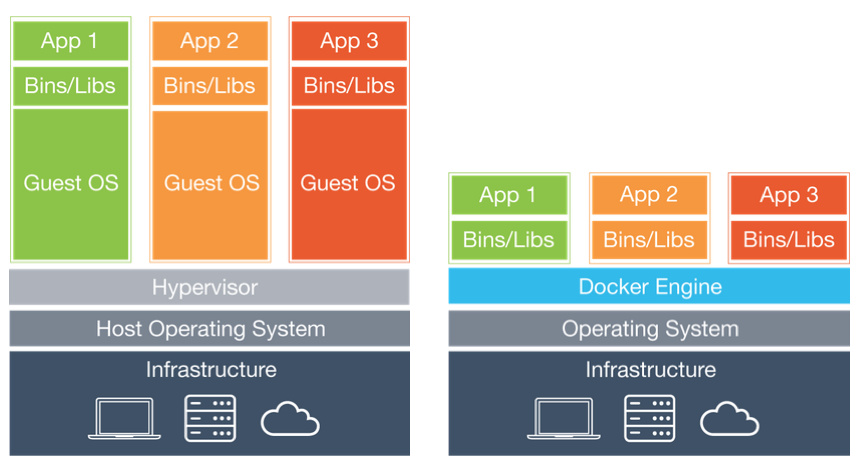
\includegraphics[width=\textwidth,keepaspectratio=true]{capitoli/imgs/ContainersvsVms.PNG}
	\caption{Confronto tra macchine virtuali e container, nell'esempio con l'utilizzo di un Docker Engine}
\end{figure}

\subsection{Vantaggi dei container}
Andiamo a ricapitolare quali sono le principali motivazioni che possono spingerci all'adozione dei container.
\begin{itemize}
	\item Coesione dell'ambiente \\
	L'ambiente di un container è fortemente disaccoppiato dalla macchina in cui si trova. Questo fà si che il proprio contenuto sia facilmente replicabile e portabile ovunque.
	
	\item Gestione delle risorse \\
	Con i containers si ha una gestione delle risorse di calcolo molto più efficiente. Richiedendo poche risorse alla macchine ospitante, si ha la possibilità di eseguire molti più container contemporaneamente. 
	
	\item Produttività \\
	Diminuendo le dipendenze, ci si alleggerisce di tutta la mole di lavoro necessaria per configurare correttamente un prodotto. 
	
	\item gestione degli aggiornamenti. \\
	Molto spesso la gestione degli aggiornamenti è un meccanismo già compreso nei container engine, come Docker.
\end{itemize}

\subsection{I container e i microservizi}
Possiamo quindi comprendere come i container siano estremamente appropriati ad ospitare del microservizi. Ponendo un microservizio dentro ogni container, abbiamo la garanzia che ogni microservizio operi come un sistema sepato, anche nell'eventualità che due servizi risiedano nella stessa macchina fisica. Ogni microservizio inserito in un container gode automaticamente di tutti i vantaggi di portabilità e flessibilità che sono tra i requisiti fondamentali che ci spingono verso l'architettura a microservizi.

\subsection{Docker}

\begin{figure}[h!]
	\centering
	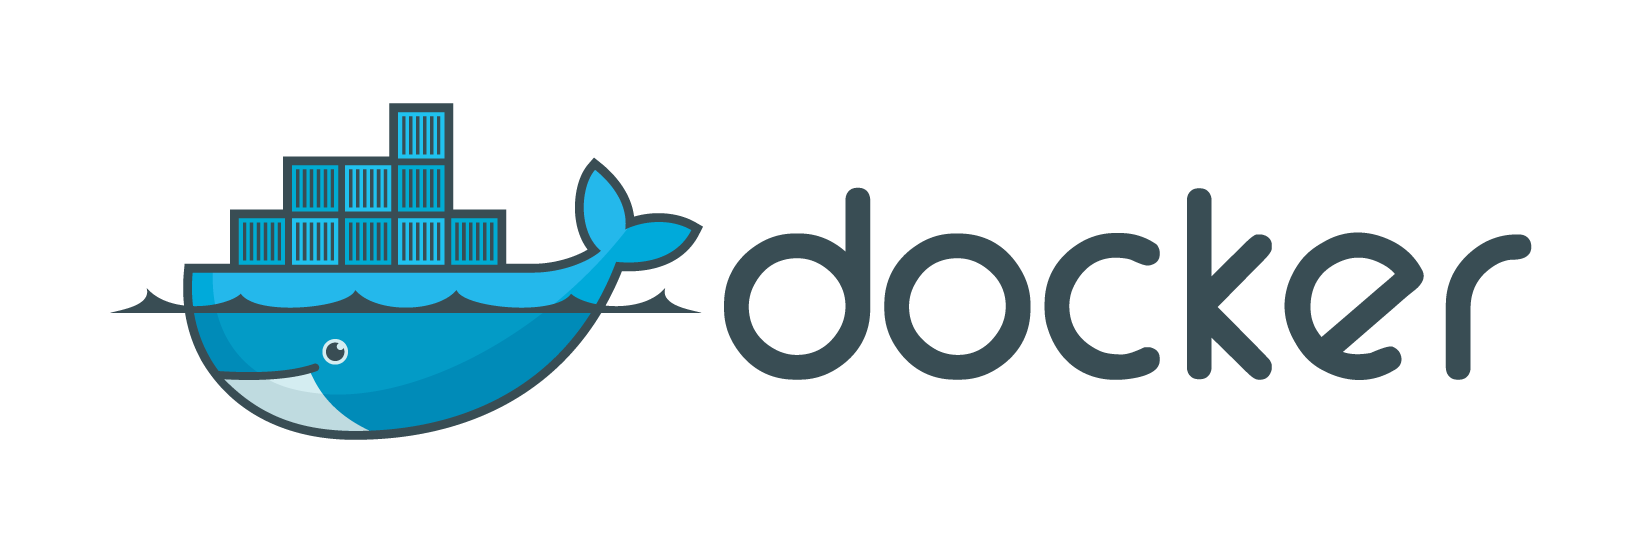
\includegraphics[width=\textwidth,keepaspectratio=true]{capitoli/imgs/docker.png}
	\caption{Logo di Docker}
\end{figure}

\subsection{Kubernetes}

\section{Multitenancy}
\section{Monitoring Tools}
\subsection{Prometheus}
\subsection{Grafana}
\section{BlueMix Service}
db2
